% Created 2016-11-14 lun 14:05
% Intended LaTeX compiler: pdflatex
\documentclass[spanish, xcolor={usenames,svgnames,dvipsnames}]{beamer}
\usepackage[utf8]{inputenc}
\usepackage[T1]{fontenc}
\usepackage{graphicx}
\usepackage{grffile}
\usepackage{longtable}
\usepackage{wrapfig}
\usepackage{rotating}
\usepackage[normalem]{ulem}
\usepackage{amsmath}
\usepackage{textcomp}
\usepackage{amssymb}
\usepackage{capt-of}
\usepackage{hyperref}
\usepackage{color}
\usepackage{listings}
\usecolortheme{rose}
\setbeamercolor{alerted text}{fg=DarkBlue}
\setbeamerfont{alerted text}{series=\mdseries}
\setbeamerfont{block title}{series=\scshape}
\setbeamercolor{block title}{bg=structure.fg!40!bg!50!bg}
\setbeamercolor{block body}{use=block title,bg=block title.bg!50}
\setbeamertemplate{navigation symbols}{}
\setbeamertemplate{blocks}[rounded][shadow=false]
\AtBeginSection[]{\begin{frame}{Índice}\tableofcontents[currentsection]\end{frame}}
\usepackage[spanish]{babel}
\usepackage{mathpazo}
\hypersetup{colorlinks=true, linkcolor=Blue, urlcolor=Blue}
\logo{\makebox[0.95\paperwidth]{
\includegraphics[width=1.5cm,keepaspectratio]{images/LogoUPM.pdf}\hfill
\includegraphics[width=1.5cm,keepaspectratio]{images/LogoETSIDI.pdf}}}
\titlegraphic{
\includegraphics[width=0.7\textwidth]{images/entrada-escuela}}
\usetheme{default}
\usefonttheme{serif}
\author{Oscar Perpiñán Lamigueiro}
\date{ETSIDI - UPM}
\title{Gestión académica de una escuela universitaria con R y shiny}
\hypersetup{
 pdfauthor={Oscar Perpiñán Lamigueiro},
 pdftitle={Gestión académica de una escuela universitaria con R y shiny},
 pdfkeywords={},
 pdfsubject={},
 pdfcreator={Emacs 24.5.1 (Org mode 9.0)}, 
 pdflang={Spanish}}
\begin{document}

\maketitle

\section{Introducción}
\label{sec:org8c3adba}

\begin{frame}[label={sec:org570d75b}]{Contexto}
\begin{itemize}
\item ETS de Ingeniería con 2700 alumnos en 10 titulaciones diferentes.
\item Numerosos grupos de matriculación (horarios).
\item Alta ocupación de aulas.
\item Planes Bolonia:
\begin{itemize}
\item Evaluación continua (frecuentes exámenes)
\item Flexibilidad de técnicas docentes
\end{itemize}
\end{itemize}
\end{frame}

\begin{frame}[label={sec:org77e4535}]{Contexto}
\begin{block}{Necesaria renovación de herramientas}
\begin{itemize}
\item Gestión de aulas
\item Elaboración y publicación de horarios docentes y calendario escolar
\item Aprobación, modificación y publicación de horarios del profesorado
\end{itemize}
\end{block}
\end{frame}


\section{Aplicaciones web}
\label{sec:org26d11f5}

\begin{frame}[label={sec:org5545fb0}]{Horarios del profesorado}
\begin{block}{Procedimiento}
\begin{itemize}
\item Cada profesor tiene un enlace único que le permite cumplimentar (y modificar) sus horarios de docencia y tutorías.
\item Cada director del departamento tiene un enlace privado para revisar estos horarios y publicarlos.
\item Una web recopila los horarios de todos los profesores, una vez publicados.
\item Otra web permite la búsqueda libre.
\end{itemize}
\end{block}
\end{frame}
\begin{frame}[label={sec:org79c570a}]{}
\begin{center}
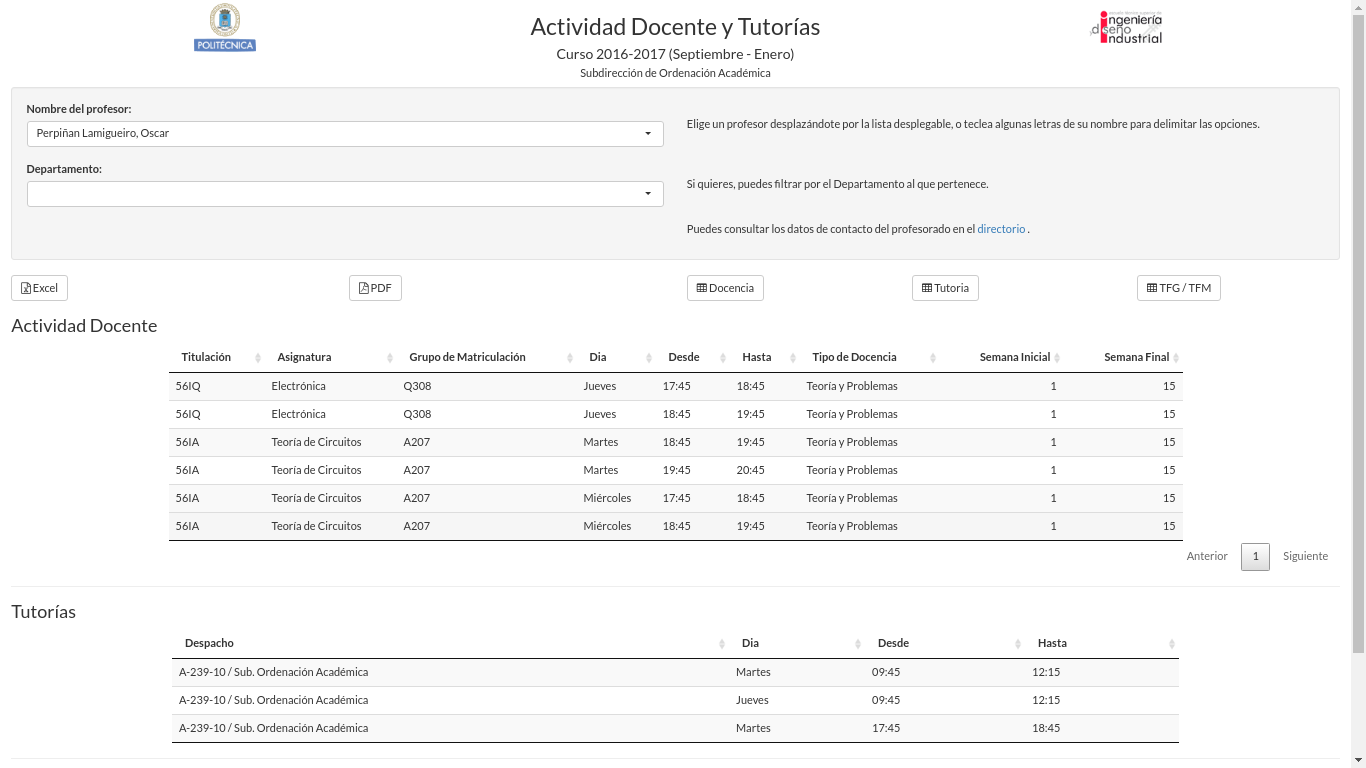
\includegraphics[width=.9\linewidth]{images/tutorias.png}
\end{center}

\url{http://programas.etsidi.upm.es/SOA/tutorias/}
\end{frame}

\begin{frame}[label={sec:orge52acd9}]{}
\begin{center}
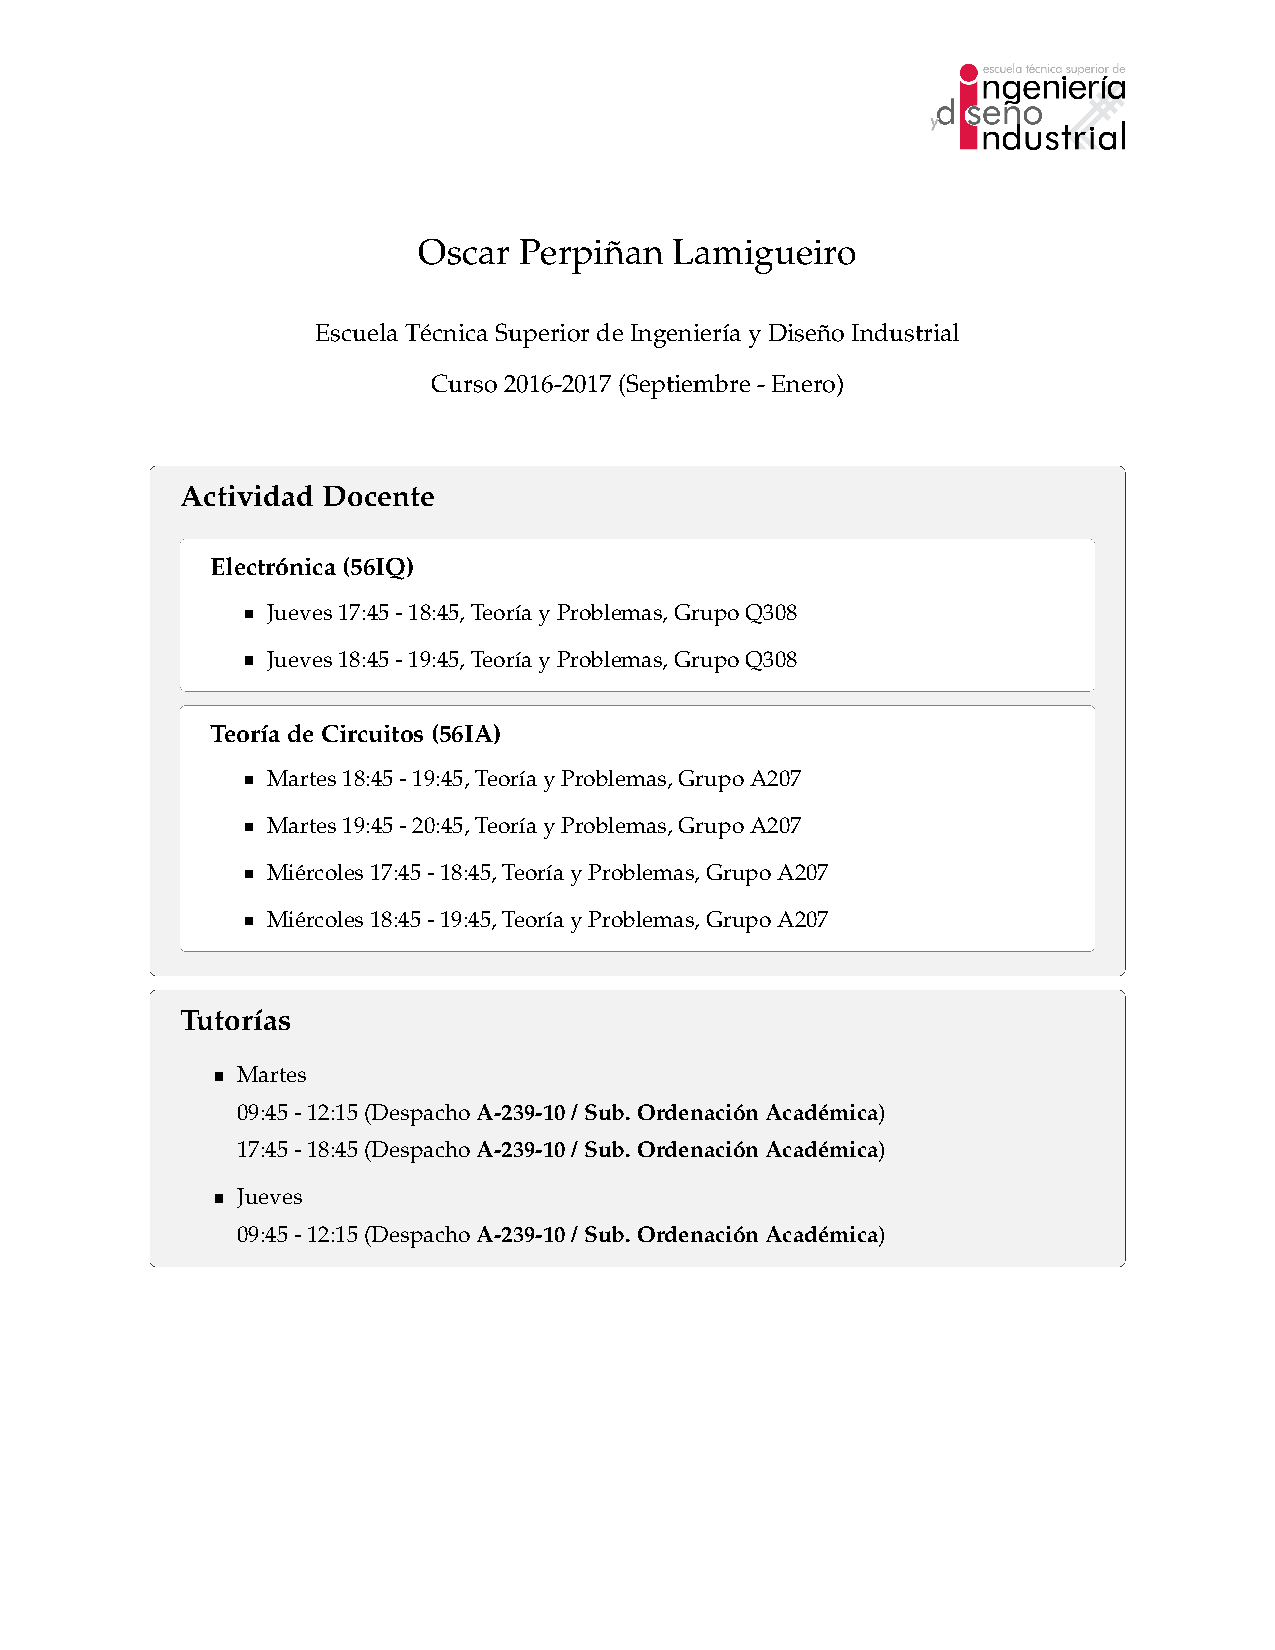
\includegraphics[width=.9\linewidth]{images/tutorias_OPL.pdf}
\end{center}
\end{frame}

\begin{frame}[label={sec:org723df11}]{}
\begin{center}
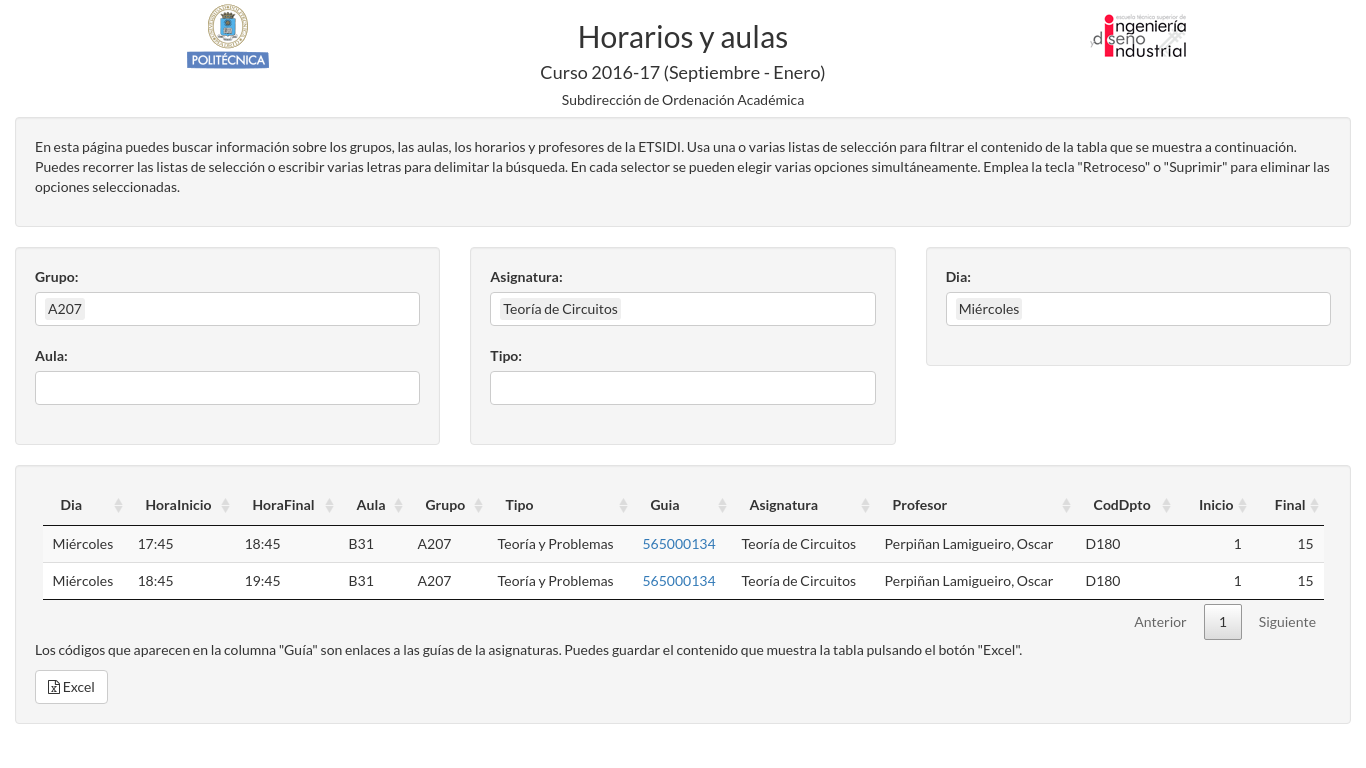
\includegraphics[width=.9\linewidth]{images/buscador.png}
\end{center}

\url{http://programas.etsidi.upm.es/SOA/buscador/}
\end{frame}

\begin{frame}[label={sec:orgf6e9853}]{Horarios del profesorado}
\begin{block}{Aspectos importantes del código}
\begin{itemize}
\item Aplicaciones basadas en shiny con la ayuda de \href{https://daattali.com/shiny/shinyjs-demo/}{shinyjs}
\item \href{https://github.com/Rdatatable/data.table/wiki}{DT} (interfaz para DataTables de JavaScript) en modo lectura y escritura (\href{https://yihui.shinyapps.io/DT-proxy/}{dataTableProxy}).
\item \href{https://github.com/Rdatatable/data.table/wiki}{data.table} detrás del escenario
\item PDF generado automáticamente a través de \href{http://orgmode.org/}{Org} (y \href{https://www.ctan.org/pkg/tcolorbox}{tcolorbox} de \LaTeX{})
\end{itemize}
\end{block}
\end{frame}
\begin{frame}[label={sec:org71b2763}]{Horarios docentes}
\begin{itemize}
\item Aplicación shiny basada en \href{http://jrowen.github.io/rhandsontable/}{rhandsontable} (tabla editable)
\item Produce:
\begin{itemize}
\item Ficheros PDF mediante \href{https://github.com/SOA-ETSIDI/horarios/blob/master/csv2tt.R}{una función} basada en una \href{https://github.com/SOA-ETSIDI/horarios/blob/master/timetable.tex}{plantilla \LaTeX{}} que usa \href{https://en.wikipedia.org/wiki/PGF/TikZ}{TikZ}
\item Ficheros iCalendar mediante dos \href{https://github.com/SOA-ETSIDI/misc/blob/master/funciones.R}{funciones propias}.
\end{itemize}
\end{itemize}
\end{frame}
\begin{frame}[label={sec:org108e578}]{}
\begin{center}
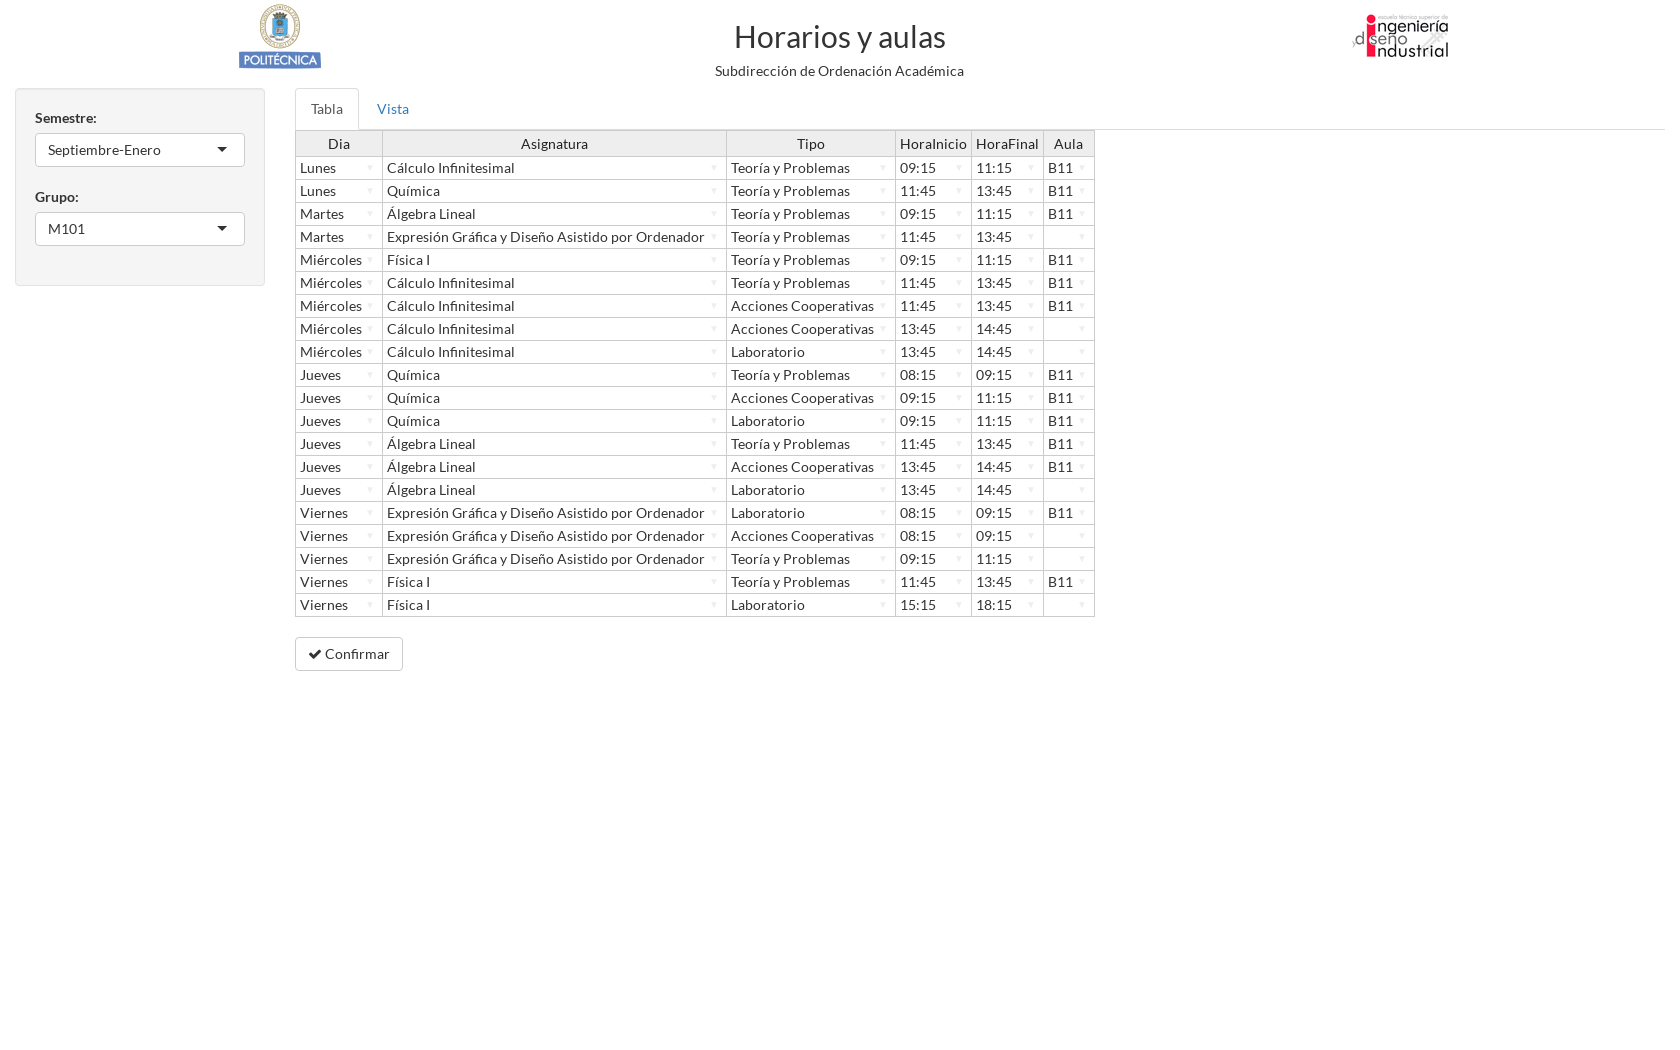
\includegraphics[width=.9\linewidth]{images/horarios.png}
\end{center}
\end{frame}

\begin{frame}[label={sec:org65f1b3a}]{}
\begin{center}
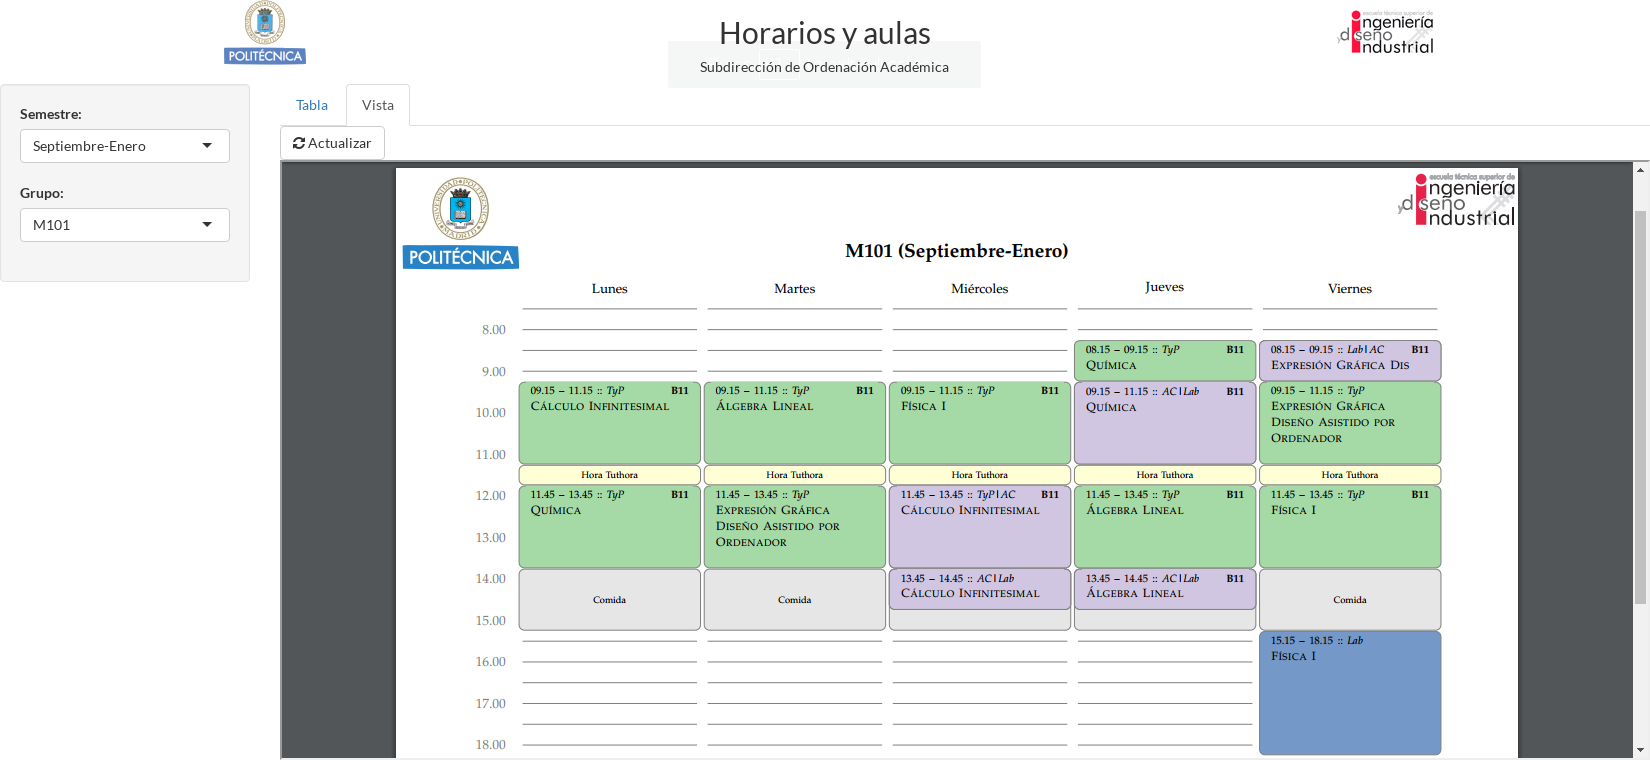
\includegraphics[width=.9\linewidth]{images/horarios_tt.png}
\end{center}
\end{frame}

\begin{frame}[label={sec:org7a07d98}]{}
\begin{center}
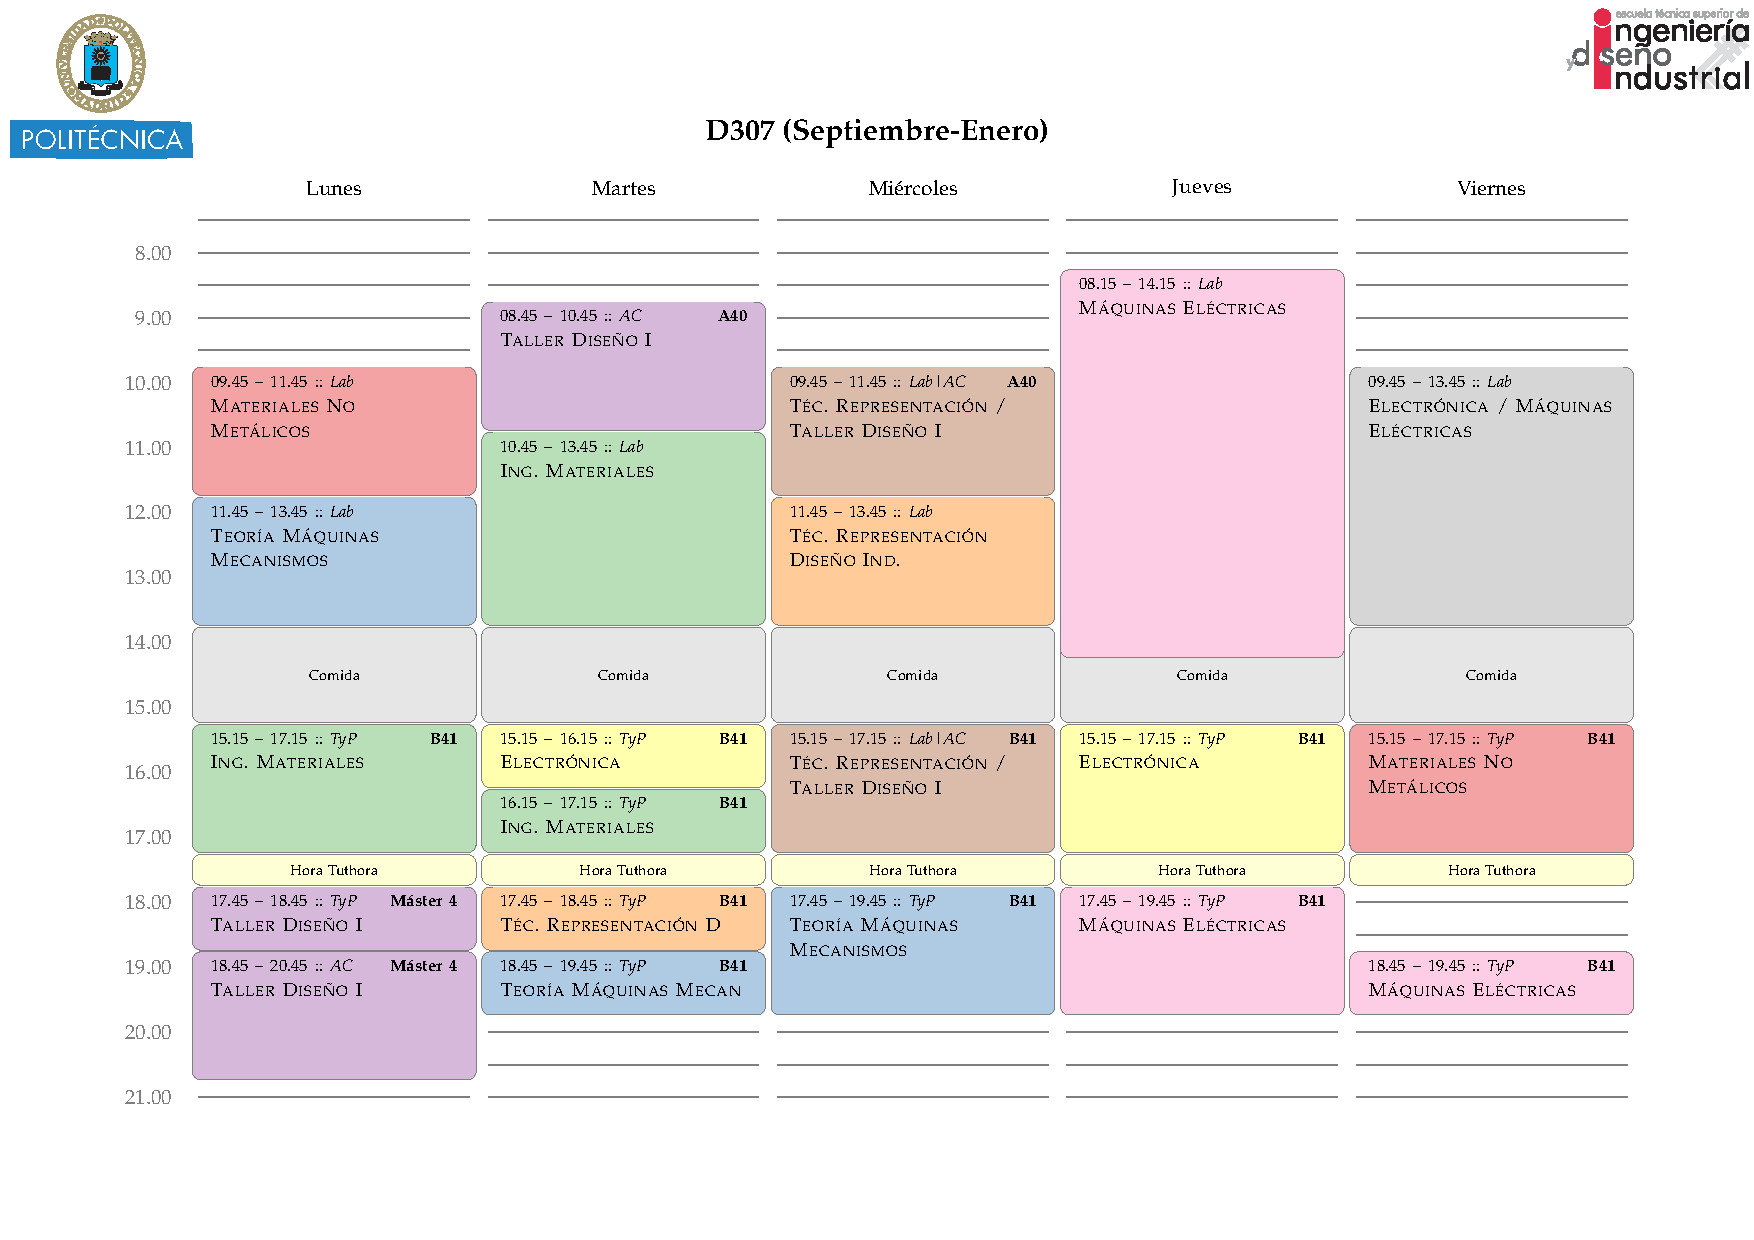
\includegraphics[width=.9\linewidth]{images/D307_1.pdf}
\end{center}

\url{http://programas.etsidi.upm.es/webdav/horarios/}
\end{frame}


\begin{frame}[label={sec:org4f4b462}]{Calendario escolar}
\end{frame}

\section{Análisis y representación de datos}
\label{sec:org01ffcde}
\end{document}